%%
%% This is file `./samples/minutes.tex',
%% generated with the docstrip utility.
%%
%% The original source files were:
%%
%% meetingmins.dtx  (with options: `minutes')
%% ----------------------------------------------------------------------
%% 
%% meetingmins - A LaTeX class for formatting minutes of meetings
%% 
%% Copyright (C) 2011-2013 by Brian D. Beitzel <brian@beitzel.com>
%% 
%% This work may be distributed and/or modified under the
%% conditions of the LaTeX Project Public License (LPPL), either
%% version 1.3c of this license or (at your option) any later
%% version.  The latest version of this license is in the file:
%% 
%% http://www.latex-project.org/lppl.txt
%% 
%% Users may freely modify these files without permission, as long as the
%% copyright line and this statement are maintained intact.
%% 
%% ----------------------------------------------------------------------
%% 
\documentclass[11pt]{meetingmins}


\usepackage{hyperref}
\usepackage{tabularx}

% To include images
\usepackage{graphicx}


%% CONFIG %%
% Default image directory
\graphicspath{{images/}}


\setcommittee{Intégration des nombres complexes et des Unum en Java avec COJAC}

\setmembers{
    Frédéric Bapst (Superviseur),
    Cédric Tâche (Etudiant)
}

\setpresent{
    Frédéric Bapst (Superviseur),
    Cédric Tâche (Etudiant)
}

\setlength{\headheight}{13.6pt}

\date{2 juin 2021}

\begin{document}

\begin {center} {
    \large \textbf {Intégration des nombres complexes et des Unum en Java avec COJAC}
}
\vspace {0.5ex}

PV de la séance du 2 juin 2020 (9h30 - 10h00) via Teams
\end {center} \vspace {1.5em}

\noindent
\textbf{Présents:} Frédéric Bapst, Cédric Tâche

\section{Ordre du jour}
Les points suivants ont été abordés durant la séance:
\begin{hiddenitems}
    \item Validation du PV du 31 mai 2021.
    \item Cahier des charges
\end{hiddenitems}

\section{PV}
\begin{hiddenitems}
    \item Le PV du 31 mai était détaillé et contenait les informations.
    \item Une phrase dans le dernier PV peut porter à confusion. Il faut implémenter au moins 1 type d'Unum, mais plusieurs types peuvent être implémentés en cas d'intérêt.
    \item Comme M. Tâche avait demandé de bons exemples de PV et que le dernier PV était bien, si une erreur apparait dans un PV suivant, l'erreur ne sera pas pénalisée la première fois.
\end{hiddenitems}

\section{Cahier des charges}
\begin{hiddenitems}
    \item Un jalon peut être ajouté dans la planification pour réaliser une démonstration des nombres complexes.
    \item D'après M. Bapst, 2 jours pourraient même suffire pour l'implémentation. Par manque d'expérience de M. Tâche avec cet outil, la durée de 4 jours déjà planifiée sera gardée.
    \item Le scénario de démonstration peut être créée plus tôt. Ça permettrait également de diriger l'implémentation vers cet objectif.
\end{hiddenitems}

\section{COJAC}
\begin{hiddenitems}
    \item Il y a des méthodes magiques dans COJAC pour accéder aux wrappers qui sont automatiquement ajouter à la place des types de base. D'autres méthodes magiques pourraient être ajoutées, notamment pour accéder aux parties réelles et imaginaires.
    \item Les branches additionnelles dur le dépôt Git proviennent des anciens projets dont presque toutes ont déjà été ajoutées au master.
    \item Il y a une erreur lors de la génération du JAR sur la machine de M. Tâche qui se produit pendant les tests.
    \item Dans la fenêtre Maven sur IntelliJ, il y a un bouton pour ne pas exécuter les tests et ainsi pouvoir générer le JAR. Ce bouton est visible sur la figure \ref{fig:skip_button}.
    \begin{figure}[ht]
        \centering
        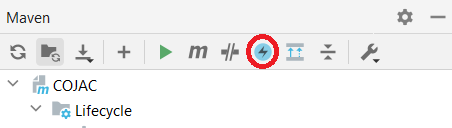
\includegraphics{skip_test_button.png}
        \caption{Bouton pour désactiver les tests}
        \label{fig:skip_button}
    \end{figure}
    \item L'objectif est tout de même de faire passer les tests.
    \item Parfois, le bouton dans IntelliJ \textbf{File > Invalidates Cache / Restart} peut corriger des problèmes avec Maven.
\end{hiddenitems}

\section{Prochaines tâches}
\begin{hiddenitems}
    \item Finir le cahier des charges.
    \item Corriger les tests qui produisent une erreur.
    \item Commencer l'analyse de COJAC.
\end{hiddenitems}

\section{Prochaines échéances}
\subsection{Responsable: M. Tâche}

\begin{table}[ht]
    \begin{tabularx}{\columnwidth}{ | X | p{8em} |}
        \hline
        \textbf{Description} & \textbf{Date limite} \\
        \hline
        Finir le cahier des charges & 07.06.2021 \\
        \hline
    \end{tabularx}
\end{table}

\vspace{1em}
\par \noindent \textbf {Prochaine séance:} Le mercredi 9 juin 2020 à 9h30

\end{document}
%% 
%% Copyright (C) 2011-2013 by Brian D. Beitzel <brian@beitzel.com>
%% 
%% This work may be distributed and/or modified under the
%% conditions of the LaTeX Project Public License (LPPL), either
%% version 1.3c of this license or (at your option) any later
%% version.  The latest version of this license is in the file:
%% 
%% http://www.latex-project.org/lppl.txt
%% 
%% Users may freely modify these files without permission, as long as the
%% copyright line and this statement are maintained intact.
%% 
%% This work is "maintained" (as per LPPL maintenance status) by
%% Brian D. Beitzel.
%% 
%% This work consists of the file  meetingmins.dtx
%% and the derived files           meetingmins.cls,
%%                                 sampleminutes.tex,
%%                                 department.min,
%%                                 README.txt, and
%%                                 meetingmins.pdf.
%% 
%%
%% End of file `./samples/minutes.tex'.
